% This is samplepaper.tex, a sample chapter demonstrating the
% LLNCS macro package for Springer Computer Science proceedings;
% Version 2.21 of 2022/01/12
%
\documentclass[runningheads]{llncs}
%
\usepackage[T1]{fontenc}
\usepackage{graphicx}
\usepackage{booktabs}
\usepackage{multirow}
\usepackage{enumitem}
\usepackage{amsmath}
\usepackage{xspace}
%
% If you use the hyperref package, please uncomment the following two lines
% to display URLs in blue roman font according to Springer's eBook style:
%\usepackage{color}
%\renewcommand\UrlFont{\color{blue}\rmfamily}
%\urlstyle{rm}
%
\newcommand{\ModelName}{GNRR\xspace}
%
\begin{document}
%
\title{Cross-Document Neural Re-Ranking via Query-Induced Subgraphs}
%
%\titlerunning{Abbreviated paper title}
% If the paper title is too long for the running head, you can set
% an abbreviated paper title here
%
\author{First Author\inst{1}\orcidID{0000-1111-2222-3333} \and
Second Author\inst{2,3}\orcidID{1111-2222-3333-4444} \and
Third Author\inst{3}\orcidID{2222--3333-4444-5555}}
%
\authorrunning{F. Author et al.}
% First names are abbreviated in the running head.
% If there are more than two authors, 'et al.' is used.
%
\institute{Princeton University, Princeton NJ 08544, USA \and
Springer Heidelberg, Tiergartenstr. 17, 69121 Heidelberg, Germany
\email{lncs@springer.com}\\
\url{http://www.springer.com/gp/computer-science/lncs} \and
ABC Institute, Rupert-Karls-University Heidelberg, Heidelberg, Germany\\
\email{\{abc,lncs\}@uni-heidelberg.de}}
%
\maketitle
%
\begin{abstract}
Neural re-rankers typically score query-document pairs independently, neglecting cross-document context within the retrieved candidate set.
We propose Graph Neural Re-Ranking (\ModelName), a framework that extracts a sparse, query-induced subgraph from a pre-computed semantic corpus graph and applies Graph Neural Networks to propagate cross-document signals.
Unlike self-attention re-rankers that scale quadratically in the number of candidates ($\mathcal{O}(K^2)$), \ModelName achieves $\mathcal{O}(c \cdot K)$ online complexity, where $c$ is the fixed corpus graph degree and $K$ the candidate set size.
On TREC-DLHard, the most challenging evaluation benchmark, \ModelName achieves up to $+5.2\%$ relative improvement in Average Precision over TCT-ColBERT and outperforms a self-attention re-ranker by $+9.0\%$ AP\@.
Notably, single-stage self-attention re-ranking \emph{degrades} performance on DLHard ($-3.5\%$ AP versus TCT-ColBERT), demonstrating that GNN propagation over corpus graphs provides complementary signal that set-based attention mechanisms fail to capture on harder queries.
A comprehensive efficiency analysis confirms that GNN models achieve these gains with fewer parameters and comparable per-query latency to self-attention, while remaining linearly scalable with candidate set size.
\end{abstract}

\keywords{Neural Re-Ranking, Graph Neural Networks, Corpus Graph}

\section{Introduction}
Modern information retrieval systems typically follow a two-stage pipeline: an initial retrieval step (e.g., BM25~\cite{bm25} or dense retrieval~\cite{colbert}) generates a set of candidate documents, which is refined by a neural re-ranking model (e.g., a transformer-based scorer~\cite{tctcolbert,vaswani2017attention}) to produce the final ranking.
Despite their effectiveness, most neural re-rankers score each query-document pair independently, discarding relationships among candidates in the retrieved set~\cite{monobert,RepBert}.

Capturing cross-document context is desirable but costly. Prior work~\cite{pang2020setrank,pobrotyn2020context,pasumarthi2020permutation} employs self-attention mechanisms over the candidate set, treating documents as a permutation-invariant set~\cite{lee2019set,pang2020setrank}. However, self-attention incurs quadratic cost $\mathcal{O}(K^2)$ in the number of documents, limiting its applicability in latency-constrained settings.
Moreover, as our experiments show, self-attention re-ranking can \emph{degrade} performance on difficult queries where relevant documents are semantically buried in the candidate set.

We take a different approach. Rather than attending over all candidate pairs, \ModelName builds a sparse, query-induced subgraph from the retrieved top-$K$ documents using a pre-computed semantic corpus graph~\cite{corpusgraph} and applies lightweight Graph Neural Networks to propagate cross-document signals. GNN message passing costs $\mathcal{O}(c \cdot K)$ online, where $c$ is the fixed corpus graph degree, linear in $K$ compared to $\mathcal{O}(K^2)$ for self-attention. Because the corpus graph is pre-computed offline, the online overhead is substantially reduced compared to dense attention-based approaches.

Our contributions are as follows:
\begin{itemize}
    \item We propose \ModelName, a re-ranking framework that applies GNN-based propagation over query-induced subgraphs to capture cross-document interactions at $\mathcal{O}(c \cdot K)$ online cost (linear in $K$ for fixed graph degree $c$), comparing favorably to the $\mathcal{O}(K^2)$ complexity of self-attention-based re-rankers.
    \item We introduce a mechanism to extract query-specific subgraphs from a large pre-computed corpus graph, enabling efficient offline-online separation.
    \item We provide a comprehensive empirical comparison of five GNN architectures against self-attention baselines across three TREC benchmarks with varying difficulty profiles. GNN-based re-ranking is uniquely robust on the hardest benchmark (DLHard), outperforming self-attention re-ranking by up to $+9.0\%$ AP while requiring linear rather than quadratic computation. We additionally report a detailed inference-time efficiency analysis.
\end{itemize}

\begin{figure}
    \centering
    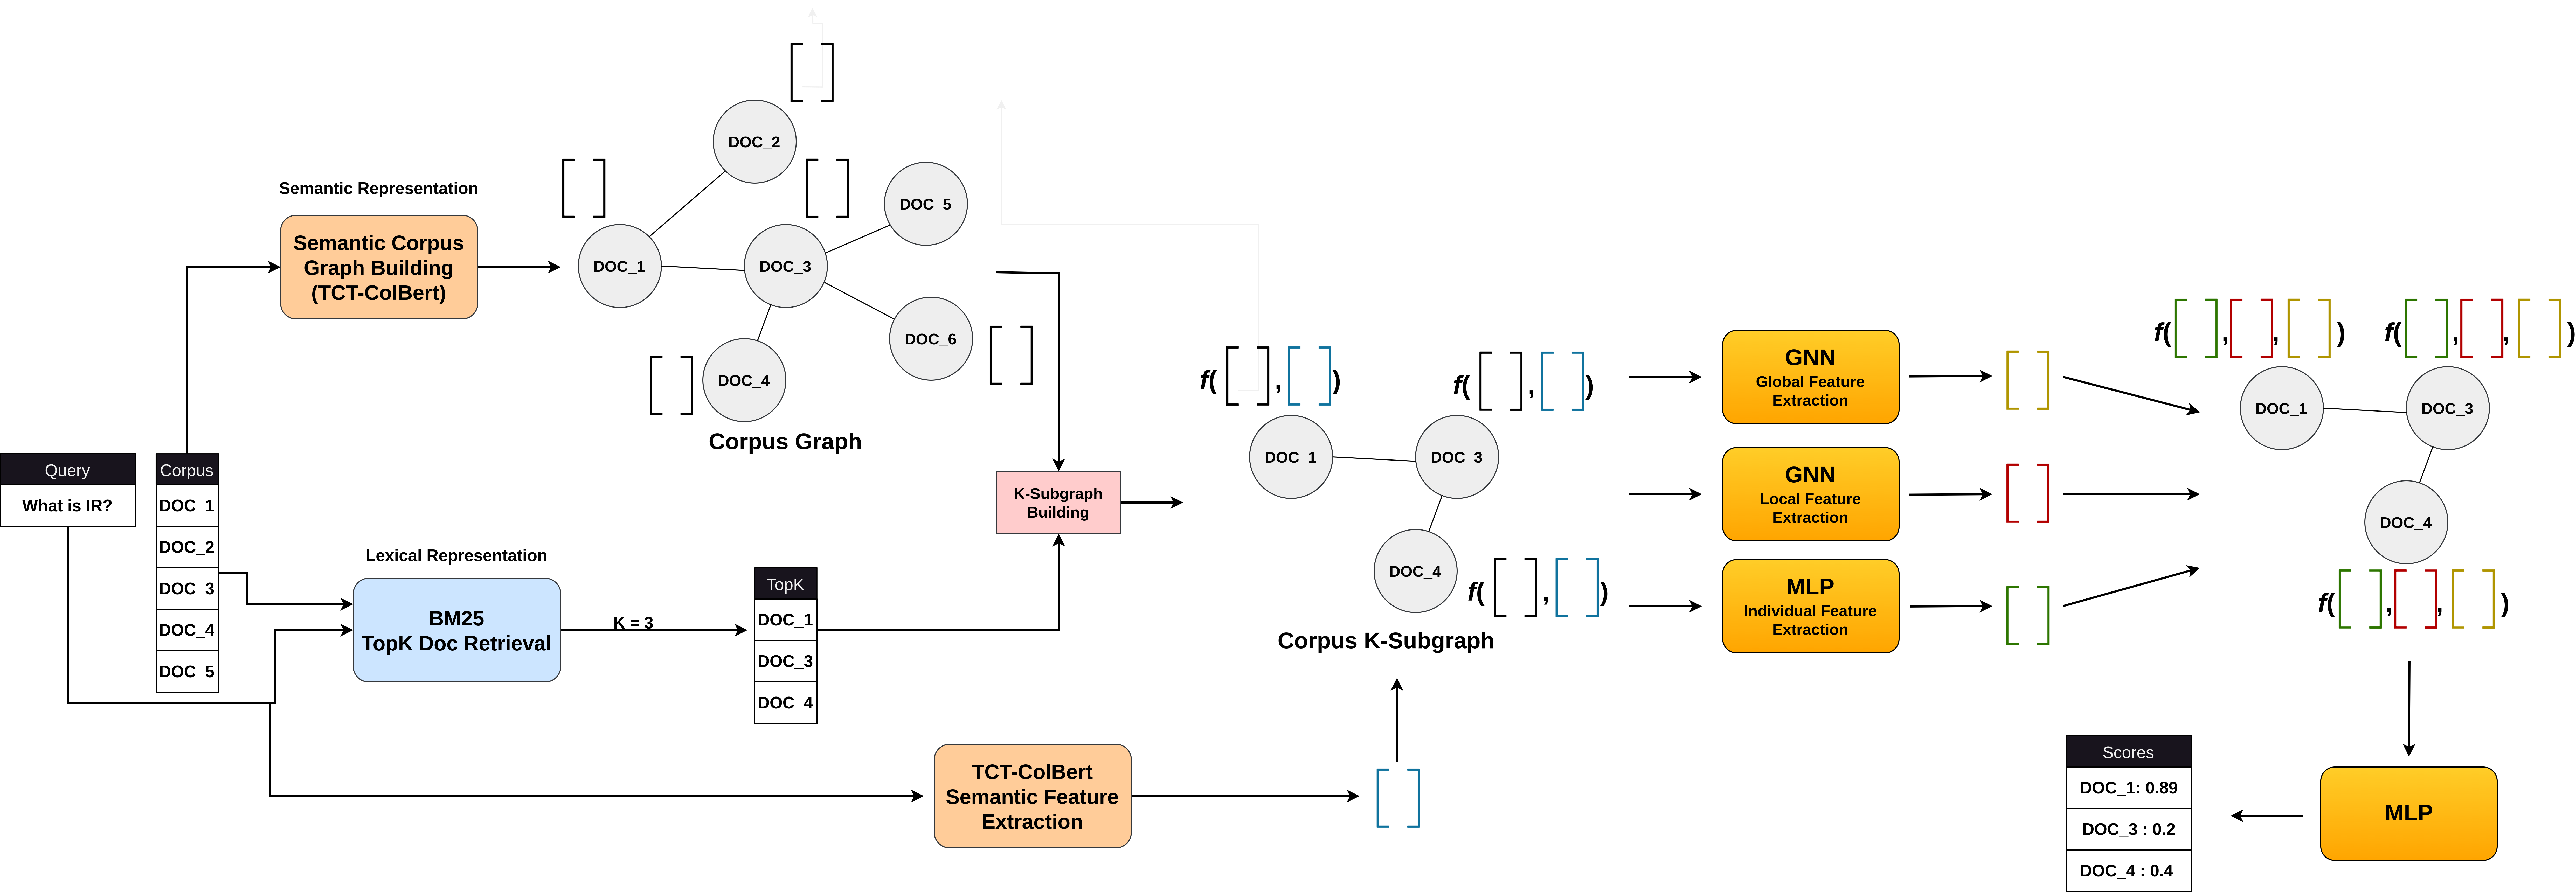
\includegraphics[width=\textwidth]{figures/general_scheme_2.png}
    \caption{Overview of \ModelName ($K=3$). \textit{Offline:} a semantic corpus graph is constructed by computing TCT-ColBERT embeddings over all documents and linking each to its $c$ nearest neighbors. \textit{Online:} given a query, (1) BM25 retrieves top-$K$ candidates; (2) TCT-ColBERT computes embeddings; (3) top-$K$ candidates induce a subgraph from the corpus graph; (4) node features are computed via $f_1(\cdot)$ from query-document embeddings; a GNN propagates cross-document signals to create contextualized representations $f_2(\cdot)$; (5) a learned scorer produces the final ranking.}
    \label{fig:overview}
\end{figure}

\section{Related Work}
Transformer-based re-rankers, such as MonoBERT~\cite{monobert}, ColBERT~\cite{colbert}, and TCT-ColBERT~\cite{tctcolbert}, rescale individual document-query relevance scores with high accuracy but treat candidates independently.

\paragraph{Set-based re-ranking.}
SetRank~\cite{pang2020setrank} and related works~\cite{pobrotyn2020context,pasumarthi2020permutation} apply self-attention over the full candidate set to capture inter-document dependencies. While effective, these methods incur $\mathcal{O}(K^2)$ cost and, as we show, can be fragile on harder query sets where relevant documents are sparsely distributed.

\paragraph{Graph-based representations in IR.}
PageRank~\cite{page1999pagerank} exemplifies how document link structure can propagate importance signals. MacAvaney et al.~\cite{corpusgraph} use a pre-computed corpus graph for graph-guided candidate expansion (GAR), showing strong retrieval improvements. \ModelName differs fundamentally: GAR augments the \emph{retrieval} stage, while \ModelName uses corpus graph structure during \emph{re-ranking}.

GNNs address this gap by jointly learning representations and propagating relevance signals across graph structure~\cite{messagepassing,everythingisconnected}. GNNs have been applied to ranking in several settings: custom PageRank from labeled examples~\cite{scarselli2005graph}, global ranking from pairwise comparisons~\cite{damke2021ranking,he2022gnnrank}, node importance in networks~\cite{liu2022learning,qu2023gnr}, and web resource ranking~\cite{ergashev2023learning}. Intra-document word graphs have also been used for relevance matching~\cite{graphofwords,graphofwords2}. Cross-document structure for re-ranking has been explored only in multi-hop QA~\cite{nie2021answeringanyhopopendomainquestions}; see~\cite{zaoad2025graphbasedrerankingemergingtechniques} for a broader survey. To our knowledge, no prior work applies GNN-based propagation over query-induced subgraphs from a pre-computed corpus graph for general-purpose document re-ranking.

\section{Methodology}
\label{sec:methodology}

\ModelName incorporates document-document relationships into neural re-ranking through three stages: (i) offline corpus graph construction, (ii) retrieval and query-induced subgraph extraction, and (iii) GNN-based re-ranking. Figure~\ref{fig:overview} illustrates the full pipeline.

\subsubsection*{\textbf{Corpus Graph}}
Given a document corpus $\mathcal{C}$, we construct an offline semantic corpus graph $\mathcal{G} = (\mathcal{C}, \mathcal{E})$ where each document $d \in \mathcal{C}$ is a node and edges $(d_i,d_j) \in \mathcal{E}$ connect semantically similar documents whose cosine similarity in the TCT-ColBERT embedding space exceeds a threshold. Each node's neighborhood is capped at a fixed cardinality $c$ to ensure sparsity. Although this offline construction is computationally expensive, it is performed only once and amortised across all queries.
We follow the construction procedure of~\cite{corpusgraph}.

\subsubsection*{\textbf{Retrieval and Subgraph Extraction}}
Given a query $q$, BM25~\cite{bm25} retrieves the top-$K$ documents $\mathcal{C}_q \subseteq \mathcal{C}$. From $\mathcal{G}$, we extract the query-induced subgraph retaining only retrieved nodes and edges between them:
\begin{equation} \label{eq:subgraph}
    \mathcal{G}_{q} = (\mathcal{C}_q, \mathcal{E}_q), \quad \mathcal{E}_q = \{(d_i,d_j) \in \mathcal{E} \;|\; d_i,d_j \in \mathcal{C}_q\}.
\end{equation}
Connectivity is bounded by construction: $|\mathcal{E}_q| \leq c \cdot K$. Each node $d_i$ is assigned a feature vector $\mathbf{x}_i = f_1(\mathbf{z}_{q}, \mathbf{z}_{d_i})$, where $\mathbf{z}_{q}, \mathbf{z}_{d_i} \in \mathbb{R}^m$ are query and document embeddings from TCT-ColBERT. The resulting feature matrix $\mathbf{X}_q \in \mathbb{R}^{|\mathcal{C}_q| \times m}$ encodes query-document relevance independently per node.

\subsubsection*{\textbf{Re-Ranking}}
The GNN operates over $\mathcal{G}_q$ to propagate cross-document signals. Each feature vector is augmented with its BM25 score to preserve lexical relevance inductive bias. The input $\mathbf{X'}_q \in \mathbb{R}^{|\mathcal{C}_q| \times (m+1)}$ is processed by the GNN:
\begin{equation}
\label{eq:local_interactions}
    \mathbf{H}_{q,\text{GNN}} = \text{GNN}(\mathbf{X'}_q, \mathbf{A}_q),
\end{equation}
where $\mathbf{A}_q$ is the adjacency matrix of $\mathcal{G}_q$ and the hidden dimension is $m'$. The GNN output is merged with the original features through a non-trainable operation $f_2$:
\begin{equation}
    \mathbf{H}_q = f_2\left(\mathbf{H}_{q,\text{GNN}}, \mathbf{X}_q\right).
\end{equation}
A scorer $\phi_{\theta}$ maps $\mathbf{H}_q$ to scalar relevance scores $\mathbf{s}_q \in \mathbb{R}^{|\mathcal{C}_q|}$, producing the final re-ranking:
\begin{equation}
    \pi_q = \text{ARGSORT}(\phi_{\theta}(\mathbf{H}_q)).
\end{equation}

\paragraph{Complexity.} By construction $|\mathcal{E}_q| \leq c \cdot K$, so GNN message passing costs $\mathcal{O}(c \cdot K)$ for fixed corpus graph degree $c$. This scales linearly with $K$, compared to $\mathcal{O}(K^2)$ for self-attention over the same candidate set.

\section{Experimental Setup}
We address three research questions:
\begin{itemize}[leftmargin=1.1cm]
\item[\textbf{RQ1.}] Does modeling cross-document interactions via GNNs improve re-ranking over a strong transformer baseline?
\item[\textbf{RQ2.}] How does GNN-based re-ranking compare to self-attention re-ranking in terms of effectiveness and efficiency?
\item[\textbf{RQ3.}] How much does the GNN branch itself contribute to the observed gains?
\end{itemize}

\subsection{Datasets}
We use the MS MARCO passage ranking corpus~\cite{msmarco} (8.8M documents). We train on 14,994 queries and validate on 200 queries from the MS MARCO training split. We evaluate on three standard test sets: TREC-DL19, TREC-DL20~\cite{dl19-20}, and TREC-DLHard~\cite{dl-hard}.
\begin{itemize}
    \item \textbf{DL19}: 43 queries, average 215 relevance judgments per query.
    \item \textbf{DL20}: 54 queries, average 211 relevance judgments per query.
    \item \textbf{DLHard}: 50 difficult queries, partially relabeled from DL19/DL20, targeting topics that challenge neural ranking models.
\end{itemize}

\subsection{Models}
We compare the following pipelines:
\begin{itemize}
    \item \textbf{BM25}~\cite{bm25}: lexical retrieval baseline.
    \item \textbf{TCT-ColBERT}~\cite{tctcolbert}: transformer-based re-ranker on top of BM25 (primary baseline).
    \item \textbf{Self-Attention}: a multi-layer Transformer encoder applied over the full BM25 candidate set features (same $f_1$ as \ModelName), trained with LambdaRank. This is an $\mathcal{O}(K^2)$ set-based re-ranker and serves as the direct efficiency comparison to \ModelName.
    \item \textbf{GAR}~\cite{corpusgraph}: graph-augmented retrieval using the same pre-computed corpus graph to expand BM25 candidates. GAR operates at the \emph{retrieval} stage (not re-ranking) and is included as a reference upper bound for corpus-graph-aware methods.
    \item \textbf{GNRR+GCN}~\cite{GCN}, \textbf{+GraphSAGE}~\cite{GraphSAGE}, \textbf{+GAT}~\cite{GAT}, \textbf{+GIN}~\cite{GIN}, \textbf{+SignedConv}~\cite{signedconv}: \ModelName variants with different GNN architectures, all using a semantic corpus graph.
\end{itemize}
We report four standard IR metrics: Average Precision (AP), Reciprocal Rank (RR), Precision at rank 3 (P@3), and nDCG@10 (rel.$\geq 2$).

\subsection{Training}
All variants are trained with LambdaRank~\cite{lambdarank}. Training runs for up to 100 epochs with early stopping on validation nDCG@10 (patience 7). The TCT-ColBERT encoder remains frozen. We report results averaged over 3 random seeds.

\subsection{Hyperparameters}
We set the corpus graph neighborhood size to $c = 16$ and $K = 1000$. The interaction function is $f_1 = \odot$ (element-wise multiplication) and the merge function is $f_2 = \|$ (concatenation). TCT-ColBERT produces embeddings of dimension $m = 768$. We tune $L \in \{1, 2, 3\}$ and $m' \in \{64, 128\}$ on the validation set.

% ---------------------------------------------------------------
% TABLE 1 — Re-ranking results (TCT-ColBERT, K=1000)
% ---------------------------------------------------------------
\begin{table}[ht]
    \centering
    \footnotesize
    \caption{Re-ranking on TREC-DL19, DL20, and DLHard using TCT-ColBERT features ($K=1000$). Self-Attention and all \ModelName variants are independent re-rankers applied on top of frozen TCT-ColBERT representations. Best score per column in \textbf{bold}. Rel.$\geq2$.}
    \vspace{0.1cm}
    \setlength{\tabcolsep}{3pt}
    \resizebox{\textwidth}{!}{%
    \begin{tabular}{lcccccccccccc}
        \toprule
        \multirow{2}{*}{\textbf{Pipeline}}
            & \multicolumn{4}{c}{\textbf{DL19}}
            & \multicolumn{4}{c}{\textbf{DL20}}
            & \multicolumn{4}{c}{\textbf{DLHard}} \\
        \cmidrule(lr){2-5} \cmidrule(lr){6-9} \cmidrule(lr){10-13}
            & AP & RR & P@3 & nDCG@10
            & AP & RR & P@3 & nDCG@10
            & AP & RR & P@3 & nDCG@10 \\
        \midrule
        BM25
            & 0.286 & 0.642 & 0.473 & 0.480
            & 0.293 & 0.619 & 0.463 & 0.494
            & 0.147 & 0.422 & 0.240 & 0.274 \\
        \addlinespace[2pt]
        +TCT-ColBERT
            & 0.430 & 0.843 & 0.667 & 0.685
            & 0.453 & 0.817 & \textbf{0.691} & 0.680
            & 0.230 & 0.538 & 0.353 & 0.373 \\
        \cmidrule(l){1-13}
        \addlinespace[1pt]
        \quad+Self-Attention
            & 0.431 & 0.844 & 0.674 & 0.686
            & 0.454 & 0.827 & 0.704 & 0.684
            & 0.222 & 0.529 & 0.340 & 0.368 \\
        \quad+GCN
            & \textbf{0.455} & \textbf{0.858} & 0.713 & \textbf{0.702}
            & \textbf{0.470} & \textbf{0.840} & 0.673 & \textbf{0.695}
            & \textbf{0.242} & \textbf{0.559} & \textbf{0.367} & \textbf{0.386} \\
        \quad+GraphSAGE
            & 0.434 & 0.850 & 0.729 & 0.689
            & 0.454 & 0.837 & 0.667 & 0.685
            & 0.223 & 0.531 & 0.367 & 0.379 \\
        \quad+GAT
            & 0.441 & 0.852 & 0.698 & 0.690
            & 0.453 & 0.826 & 0.685 & 0.682
            & 0.219 & 0.542 & 0.367 & 0.376 \\
        \quad+GIN
            & 0.449 & 0.853 & \textbf{0.729} & 0.691
            & 0.455 & 0.793 & 0.642 & 0.675
            & 0.215 & 0.490 & 0.333 & 0.357 \\
        \quad+SignedConv
            & 0.426 & 0.828 & 0.698 & 0.675
            & 0.445 & 0.813 & 0.685 & 0.676
            & 0.218 & 0.509 & 0.353 & 0.366 \\
        \bottomrule
    \end{tabular}%
    }
    \label{tab:benchmarking}
\end{table}

% ---------------------------------------------------------------
% TABLE 2 — Effect of improved recall: GAR + GNRR re-ranking
% ---------------------------------------------------------------
\begin{table}[ht]
    \centering
    \footnotesize
    \caption{Effect of improved retrieval recall on re-ranking. GAR augments BM25 candidates with semantic-graph-neighbor documents; \ModelName re-rankers (trained on BM25 pools) are applied to the GAR-enlarged pool without retraining, using the same semantic corpus graph as during training. Best per column in \textbf{bold}. Rel.$\geq2$.}
    \vspace{0.1cm}
    \setlength{\tabcolsep}{3pt}
    \resizebox{\textwidth}{!}{%
    \begin{tabular}{lcccccccccccc}
        \toprule
        \multirow{2}{*}{\textbf{Pipeline}}
            & \multicolumn{4}{c}{\textbf{DL19}}
            & \multicolumn{4}{c}{\textbf{DL20}}
            & \multicolumn{4}{c}{\textbf{DLHard}} \\
        \cmidrule(lr){2-5} \cmidrule(lr){6-9} \cmidrule(lr){10-13}
            & AP & RR & P@3 & nDCG@10
            & AP & RR & P@3 & nDCG@10
            & AP & RR & P@3 & nDCG@10 \\
        \midrule
        BM25
            & 0.286 & 0.642 & 0.473 & 0.480
            & 0.293 & 0.619 & 0.463 & 0.494
            & 0.147 & 0.422 & 0.240 & 0.274 \\
        +TCT-ColBERT
            & 0.430 & 0.843 & 0.667 & 0.685
            & 0.453 & \textbf{0.817} & \textbf{0.691} & 0.680
            & 0.230 & \textbf{0.538} & 0.353 & 0.373 \\
        \cmidrule(l){1-13}
        \addlinespace[1pt]
        GAR (retrieval augmentation)
            & 0.440 & 0.833 & 0.667 & 0.696
            & 0.447 & 0.815 & 0.685 & 0.680
            & \textbf{0.233} & 0.532 & 0.353 & \textbf{0.373} \\
        \addlinespace[2pt]
        \quad+GCN (re-ranking on GAR pool)
            & 0.419 & 0.824 & 0.698 & 0.692
            & 0.422 & 0.785 & 0.630 & 0.647
            & 0.224 & 0.519 & \textbf{0.360} & 0.353 \\
        \quad+GraphSAGE
            & 0.431 & 0.815 & 0.698 & 0.697
            & 0.432 & 0.790 & 0.667 & 0.664
            & 0.220 & 0.501 & \textbf{0.360} & 0.356 \\
        \quad+GAT
            & \textbf{0.444} & 0.833 & \textbf{0.721} & \textbf{0.705}
            & \textbf{0.458} & 0.808 & 0.679 & \textbf{0.681}
            & 0.229 & 0.495 & \textbf{0.360} & 0.368 \\
        \quad+GIN
            & 0.429 & 0.790 & 0.674 & 0.676
            & 0.421 & 0.777 & 0.617 & 0.616
            & 0.200 & 0.456 & 0.320 & 0.325 \\
        \quad+SignedConv
            & 0.420 & \textbf{0.846} & 0.690 & 0.687
            & 0.413 & 0.786 & 0.623 & 0.657
            & 0.212 & 0.501 & 0.347 & 0.347 \\
        \bottomrule
    \end{tabular}%
    }
    \label{tab:gar_gnrr}
\end{table}

\section{Results}

\subsection{GNN Re-Ranking vs.\ TCT-ColBERT (RQ1)}

Table~\ref{tab:benchmarking} shows that GNN re-ranking improves over TCT-ColBERT for the most effective architectures, with notable variation across models and benchmarks. GCN achieves the strongest and most consistent improvements: $+5.8\%$ AP on DL19, $+3.8\%$ on DL20, and $+5.2\%$ on DLHard, with nDCG@10 gains of $+2.5\%$, $+2.2\%$, and $+3.5\%$ respectively. GraphSAGE also improves positively on DL19 ($+0.9\%$ AP) and DLHard ($+1.3\%$). GAT and GIN show notable gains on DL19 ($+2.6\%$ and $+4.4\%$) but degrade on DLHard ($-4.8\%$ and $-6.5\%$), while SignedConv falls slightly below TCT-ColBERT across all three benchmarks.

The DLHard benchmark is most revealing: GCN raises AP from $0.230$ to $0.242$ ($+5.2\%$) and nDCG@10 from $0.373$ to $0.386$ ($+3.5\%$), and GraphSAGE also improves, while architectures with less robust aggregation (GAT, GIN, SignedConv) degrade on this harder setting. This bifurcation suggests that graph-based cross-document propagation is particularly beneficial when pointwise scoring struggles, but that the choice of aggregation scheme significantly influences generalization to harder query distributions.

\subsection{GNN vs.\ Self-Attention (RQ2)}

\paragraph{Effectiveness.}
Table~\ref{tab:benchmarking} reveals a striking asymmetry between GNN-based and self-attention re-ranking.
On DL19, single-stage self-attention marginally improves over TCT-ColBERT ($+0.2\%$ AP), comparable to GNN models.
On DL20, both self-attention and GNN models offer modest gains, suggesting that DL20 queries are largely well-addressed by pointwise scoring.
On \textbf{DLHard}, however, self-attention \emph{degrades} TCT-ColBERT performance by $-3.5\%$ AP ($0.222$ vs.\ $0.230$) and $-1.3\%$ nDCG@10. In the same setting, GCN and GraphSAGE consistently improve over TCT-ColBERT. Compared directly to single-stage self-attention, GCN achieves $+9.0\%$ AP on DLHard ($0.242$ vs.\ $0.222$).

We attribute this asymmetry to structural regularization: the sparse corpus graph constrains information flow to semantically similar document pairs, while the full $K\!\times\!K$ attention matrix over predominantly non-relevant candidates amplifies noise in hard-query settings. The GNN, by attending only to corpus-graph neighbors, effectively filters out irrelevant cross-document interactions.

\paragraph{Inference efficiency (Table~\ref{tab:efficiency}).}
\begin{table}[ht]
    \centering
    \footnotesize
    \caption{Inference efficiency at $K=1000$. Latency averaged over DL19 queries on NVIDIA RTX 3090 Ti (GNN forward pass + subgraph extraction; TCT encoding excluded). GNN methods cost $\mathcal{O}(c \cdot K)$ with $c=16$ fixed, versus $\mathcal{O}(K^2)$ for self-attention.}
    \vspace{0.1cm}
    \setlength{\tabcolsep}{4pt}
    \begin{tabular}{lrrr}
        \toprule
        \textbf{Method} & \textbf{Complexity} & \textbf{Params} & \textbf{ms/query} \\
        \midrule
        Self-Attention       & $\mathcal{O}(K^2)$         & 363.9K & 37.3 \\
        \midrule
        GNRR+GCN       & $\mathcal{O}(c \cdot K)$   & 263.0K & 34.2 \\
        GNRR+GraphSAGE & $\mathcal{O}(c \cdot K)$   & 160.2K & 32.8 \\
        GNRR+GAT       & $\mathcal{O}(c \cdot K)$   & 246.8K & 34.3 \\
        GNRR+GIN       & $\mathcal{O}(c \cdot K)$   & 123.5K & 32.4 \\
        GNRR+SignedConv & $\mathcal{O}(c \cdot K)$  & 295.7K & 35.2 \\
        \bottomrule
    \end{tabular}
    \label{tab:efficiency}
\end{table}

GNN models are simultaneously faster and smaller than self-attention: at $K=1000$, GNN latency is $6$--$13\%$ lower (32--35~ms vs.\ 37.3~ms) with up to $66\%$ fewer parameters (GIN: 124K vs.\ 364K). The advantage grows with $K$: self-attention cost scales as $\mathcal{O}(K^2)$, so doubling $K$ quadruples its cost while GNN cost grows as $\mathcal{O}(c \cdot K)$ and remains linear. GNN models therefore achieve better DLHard effectiveness at lower computational cost.

\subsection{Sensitivity to Candidate Distribution (supplementary)}\label{sec:gar}

Table~\ref{tab:gar_gnrr} examines what happens when \ModelName re-rankers (trained on BM25 candidate pools) are applied to GAR-augmented pools without retraining, using the same semantic corpus graph as during training.
GAR improves the retrieval stage over the TCT-ColBERT baseline: on DL19, AP rises from $0.430$ to $0.440$ ($+2.3\%$) and nDCG@10 from $0.685$ to $0.696$, by graph-guided candidate expansion alone.

The five \ModelName architectures respond differently to this distribution shift.
GCN, GIN, GraphSAGE, and SignedConv all degrade AP relative to GAR alone across all three benchmarks, confirming a classic out-of-distribution failure: these models were trained to re-rank BM25 candidate pools and their fixed, non-adaptive aggregation schemes do not transfer directly to the larger, more diverse candidate distribution produced by GAR.
\textbf{GAT is the exception on DL19 and DL20.} Its attention mechanism can adaptively reweight neighbors at test time, improving AP over GAR alone by $+0.9\%$ on DL19 ($0.444$ vs.\ $0.440$) and $+2.5\%$ on DL20 ($0.458$ vs.\ $0.447$); GAT also records the best nDCG@10 on both benchmarks. On DLHard, all five architectures degrade, suggesting that the shift in candidate distribution is particularly challenging on harder queries regardless of aggregation scheme.

These results carry two messages. First, attention-based aggregation generalizes better across candidate distributions than isotropic GNN operators on typical queries. Second, the retrieval and re-ranking stages must be jointly calibrated when the candidate source changes; re-training \ModelName on GAR-augmented training pools is a natural avenue for future work.

\subsection{GNN Branch Contribution (RQ3)}

Table~\ref{tab:benchmarking} isolates the GNN contribution by comparing each \ModelName variant against the TCT-ColBERT baseline. GCN achieves nDCG@10 gains of $+2.5\%$ on DL19, $+2.2\%$ on DL20, and $+3.5\%$ on DLHard, confirming that learned message passing over query-induced subgraphs provides ranking signal that pointwise query-document representations do not capture. GCN is the most robust architecture, improving across all three benchmarks; GraphSAGE follows on DL19 and DLHard. GAT and GIN achieve notable gains on DL19 but are less robust on DLHard, while SignedConv consistently underperforms TCT-ColBERT. These results suggest that the choice of GNN aggregation scheme significantly influences generalization across query difficulty profiles, a finding that connects to the GAR transfer experiment (Section~\ref{sec:gar}), where attention (GAT) proves more robust to candidate distribution shift on standard queries.

\section{Conclusions}
This paper introduced \ModelName, a re-ranking framework that captures cross-document interactions by extracting a sparse, query-induced subgraph from a pre-computed semantic corpus graph and applying a GNN over transformer-based representations. Unlike self-attention re-rankers with $\mathcal{O}(K^2)$ cost, \ModelName requires only $\mathcal{O}(c \cdot K)$ online computation, linear in the candidate set size for fixed corpus graph degree $c$.

A comprehensive comparison with self-attention re-ranking reveals that GNN-based methods are uniquely robust on harder query sets: on TREC-DLHard, GCN achieves $+5.2\%$ AP over TCT-ColBERT and $+9.0\%$ AP over self-attention, whereas single-stage self-attention \emph{degrades} performance below the TCT-ColBERT baseline on the same set. Inference-time analysis confirms that GNN models achieve this with fewer parameters and lower per-query latency at $K=1000$, with a theoretical linear vs.\ quadratic scaling advantage as $K$ grows.

These results establish that sparse inter-document structure via pre-computed corpus graphs is a viable and computationally efficient mechanism for improving neural re-ranking, with particular value for difficult retrieval scenarios.

\subsection*{Limitations and Future Work}
Results are mixed on DL20, suggesting that not all query distributions benefit equally from graph propagation. Future work includes: (1) heterogeneous graph structures encoding multiple relation types; (2) joint training with the dense encoder; (3) adaptive graph construction per query; and (4) scaling the corpus graph neighborhood size and studying its interaction with re-ranking quality. The gap between GAR (corpus-graph retrieval augmentation) and \ModelName (re-ranking) also suggests that combining both approaches with joint training is a natural direction.

\begin{credits}
\subsubsection{Generative AI Usage Disclosure}
Generative AI tools were used for debugging assistance and language editing only. Conceptualization, methodology, experimental design, analysis, and manuscript writing were conducted entirely by the authors.

\subsubsection{\discintname}
The authors have no competing interests to declare that are relevant to the content of this article.
\end{credits}

%
% ---- Bibliography ----
%
\bibliographystyle{splncs04}
\bibliography{main}
\end{document}
